\documentclass{article}

\usepackage{titlesec}

\usepackage{amsmath}
\usepackage{amssymb}

\usepackage{booktabs}
\usepackage{float}
\usepackage{colortbl}
\usepackage{xcolor}

\usepackage{a4wide}
\usepackage{setspace}
\usepackage{geometry}
\usepackage{parskip}

\usepackage{graphicx}
\graphicspath{ {../figures/} }

\usepackage[style=chicago-authordate,backend=biber]{biblatex}
\addbibresource{samplebib.bib}

\usepackage{hyperref}
\hypersetup{
    colorlinks=true,
    linkcolor=black,
    urlcolor=blue
}

\author{Yu Xia}
\title{Does Prison Construction Lead to Reduction on Crime?}
\date{Spring 2022}

\begin{document}
\maketitle

\nocite{*}

\begin{abstract}
    This paper estimates the causal effect of prison construction on the rate of crime in Texas by measuring ATT. It uses the state-level data between 1985 and 2000, and fits the pre-trend of crime rate before the prison construction. The paper then predicts post-trend using synthetic control. Results imply that the implementation reduces the crime rate by above 1\%, but the impact of prison construction is getting weaker in the long-term. The results also show that the prison construction has an insignificant effect on reducing crime rate. In conclusion, constructing prisons should not be the only way to reduce crime, and it's better to be conservative about the synthetic control method.
\end{abstract}

\section{Introduction}

In the past decades, incarceration in the US has gone high. Intuitively, the more incarceration, the less crimes are. But is it really the case? To have a clearer picture, this paper looks at the causal effect of incarceration on the rate of crimes and the extent of it. Using synthetic control, this paper estimates the rate of crime in the synthetic world. What this paper cares about is the ``gap" (that is, the ATT) between the actual world and synthetic world, in terms of the crime rate. By discussing the result, this paper might be helpful in providing some ideas about how to reduce the rate of crime. 

The remaining parts of this paper is organized as follows: The next section talks about the background of this problem. Then this paper describes the data and the method used to estimate. The fourth section provides the comparison of actual and synthetic cases, discussing the result. Finally, the paper provides some remarks.

\section{Background}

In the 1980s, the Texas government lost its case related to overcrowded prison condition. At that time, what Texas could do was to grant more parole. But then, especially in about 1993, Texas began to increase the capacity of prisons. As a result, Texas grants less parole, and the incarceration rate increases. It's unclear, however, whether more incarceration will lead to a lower crime rate. 

A higher incarceration rate may keep felons inside the prison, and has both incapacitation and deterring effect on crime. Weisburd, Einat, and Kowalski (2008) suggested that fine payment has a deterrent effect, monetary penalties for probation could be regarded as an alternative of incarceration. Ross (1984) noted that stricter laws reduce drinking and driving. According to Helland and Tabarrok (2007), California's three-strikes law reduced the felony arrest rate. But Iyengar's analysis (2008) shows that ``The high cost of incarceration combined with the high cost of violent crime relative to non-violent crime implies that Three Strikes may not be a cost-effective means of reducing crime." There are also plenty of articles looking at incarceration. Abrams (2012) estimated the deterrent effect of incarceration and got robust results. Under prison overcrowding litigation, Levitt (1996) showed that incarcerating one more prisoner reduces the number of crimes by approximately 15 per year, and the marginal costs of incarceration were below the accompanying social benefits of crime reduction. 

Some papers point out that incarceration may not be very useful in decreasing crime rate. The reduction in California's incarceration rate had just a modest effect on property crimes, and little effect on violent effect (Lofstrom, and Raphael 2016). Kuziemko (2013) estimated the effect of eliminating parole, suggesting that parole might be a good alternative compared to incarceration. For teenagers' peer effect, Bayer et al. (2009) and Ouss (2013) both found strong evidence, in terms of recidivism. Drago and Galbiati (2012) used an Italian experiment, and showed that peer effects tend to have a strong impact on criminal behavior. Additionally, teenagers are easier to be influenced by bad behavior when in prison, and join the gang or choose crime in the future. There are also literatures talking about gangs (Hunt et al. 1993; Moore et al. 1978; Vigil 1989). Those people in the prison may organize gangs, and after they are released, these gangs may harm the local community (Moore 1996). 

As the number of people in prison increases, the potential negative effects of incarceration could be higher. Hence, the actual effect of incarceration is not as easy to tell as intuition. 


\section{Data}

The crime data comes from Uniform Crime Reports (ICPSR) from the FBI. The population of each state is recorded in the dataset of Center for Disease Control (CDC). Other state level variables could be collected from the Current Population Survey (CPS). This paper also refers to Cunningham (2021) and Abadie, Diamond and Hainmueller (2010). The data spans from 1985 to 2000.

Table 1 provides a summary table of some key variables. 

\input{../Tables/Table_1.tex}

\section{Model}

The synthetic control estimator measures:
$$
    Y_{1t} - \sum_{j=2}^{J+1} w_j^* Y_{jt}
$$

where \( \mathnormal{Y_{jt}} \) is the crime rate at \( \mathnormal{t} \) for state \( \mathnormal{j} \). Particularly, \( \mathnormal{Y_{1t}} \) represents the crime rate of Texas at time \( \mathnormal{t} \) in this equation. The algorithm will use the state FIPS codes instead. The estimator specifies weights \( \mathnormal{w_j^*} \) in order to predict Texas's crime rate as real as possible. 

The synthetic control estimator chooses matrix \( \mathnormal{V} \), such that minimizes the mean square error:

$$
   \sum_{t=2}^{T_0} \left[Y_{1t} - \sum_{j=2}^{J+1} w_j^* (V) Y_{jt} \right]^2 
$$

The potential assumption is that the sum of weights is equal to 1, and each weight is non-negative. This paper regards the significant increase of prison construction in 1993 as the treatment event. By using synthetic control, if the trend before treatment happens fits well, it is assumed that the synthetic trend to be the trend of Texas without treatment. 
\newpage

\section{Analysis}

This paper puts 2 different weights on synthetic control. For the first time, the estimation is based on variables related to crime. The second estimation makes use of variables that indirectly influence the crime rate, such as labor market indicators, income indicators. By using R, the synthetic control algorithm minimizes the squared error before the treatment event happens, and predicts post-trend accordingly. 

Figure 1 shows the outcome of trends comparison. 

\begin{figure}[H]
    \begin{center}
        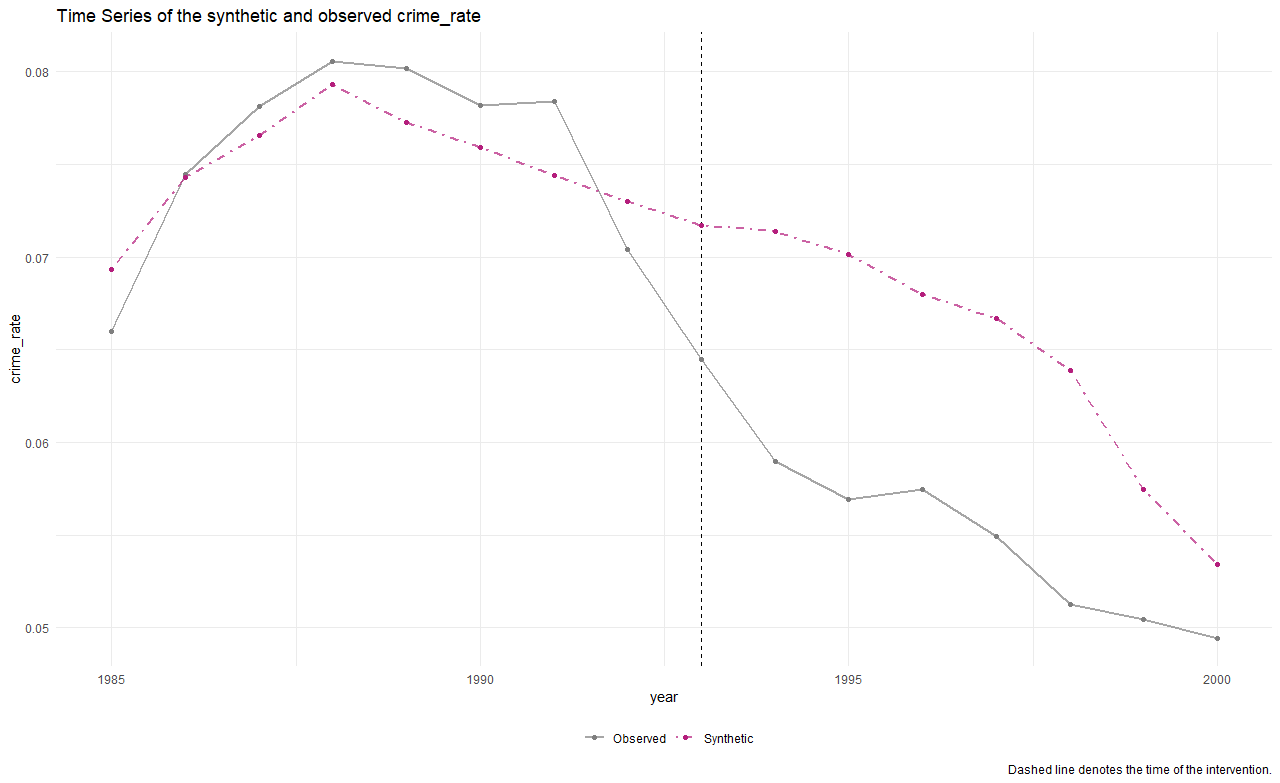
\includegraphics[width=.85\textwidth]{Figures/figure_1.png}
    \end{center}
    \caption{Trend Comparison}
    \label{fig:graph}
\end{figure}

As figure 1 shows, the treatment seemingly comes to effect in the beginning, but the effect in the real world converges to the synthetic case as time goes by. 

Figure 2 highlights the gap between the actual and synthetic Texas.

As the figure 2 shows, the crime rate reduces more than 1\% in 10 years. But this effect diminished 10 years after the prison was constructed. It's similar with Abrams's (2012) and Levitt's (1996) results.


\begin{figure}[H]
    \begin{center}
        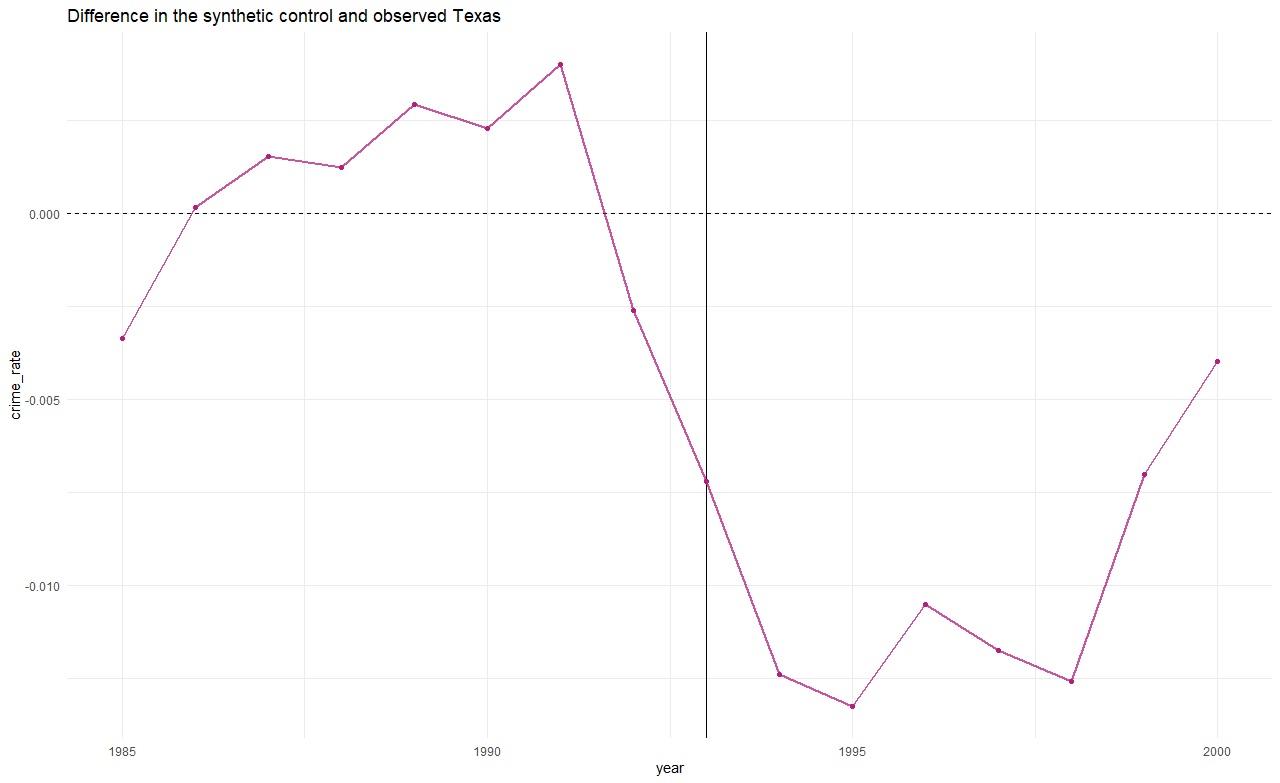
\includegraphics[width=.85\textwidth]{Figures/figure_2.png}
    \end{center}
    \caption{Gap Comparison}
    \label{fig:graph}
\end{figure}


Table 2 and Figure 3 shows the weight of states and variables in the first synthetic estimation.

\input{../Tables/Table_2.tex}

\begin{figure}[H]
    \begin{center}
        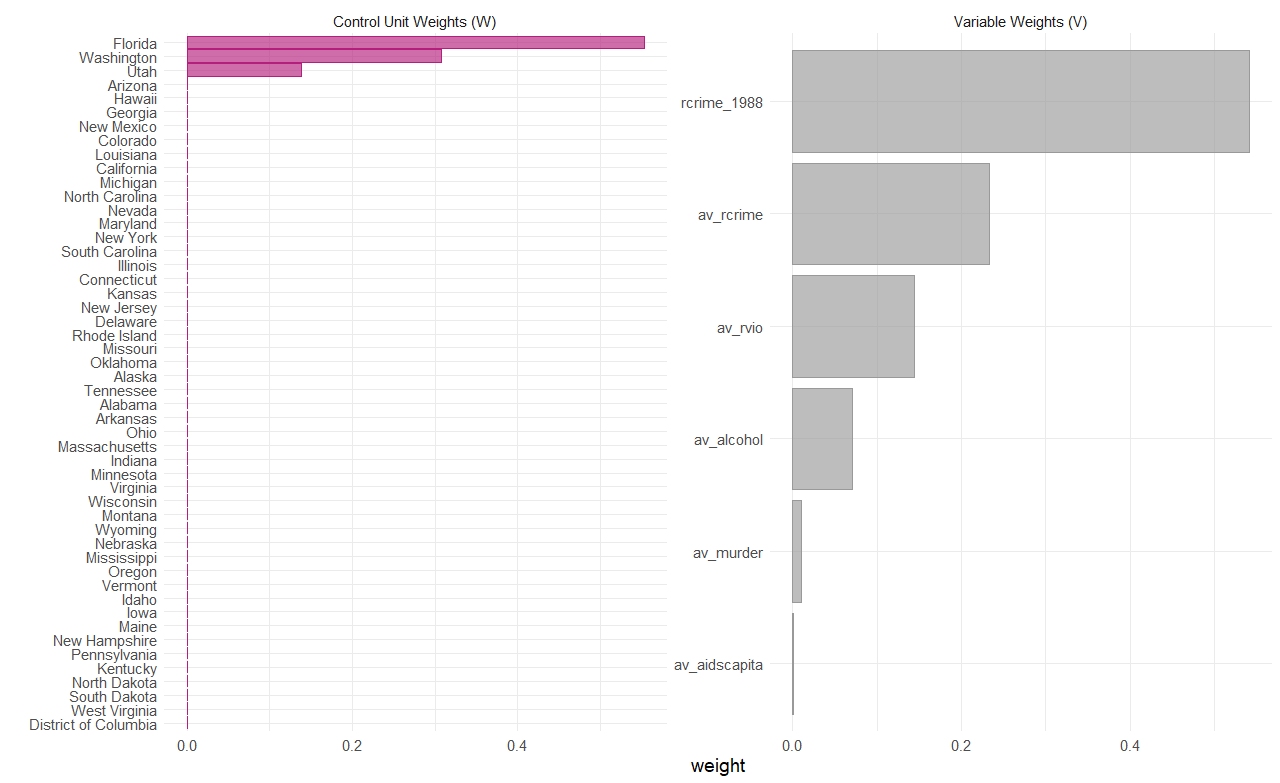
\includegraphics[width=.85\textwidth]{Figures/figure_3.png}
    \end{center}
    \caption{Synthetic Control Weights (before adding variables)}
    \label{fig:graph}
\end{figure}

Some variables, such as unemployment rate, incomes, are indirectly related to crime rate. Taking them into consideration, estimate again. The trend and gap don't vary too much from Figure 1 and 2. Table 3 and Figure 4 shows the weights. 

\input{../Tables/Table_3.tex}

\begin{figure}[H]
    \begin{center}
        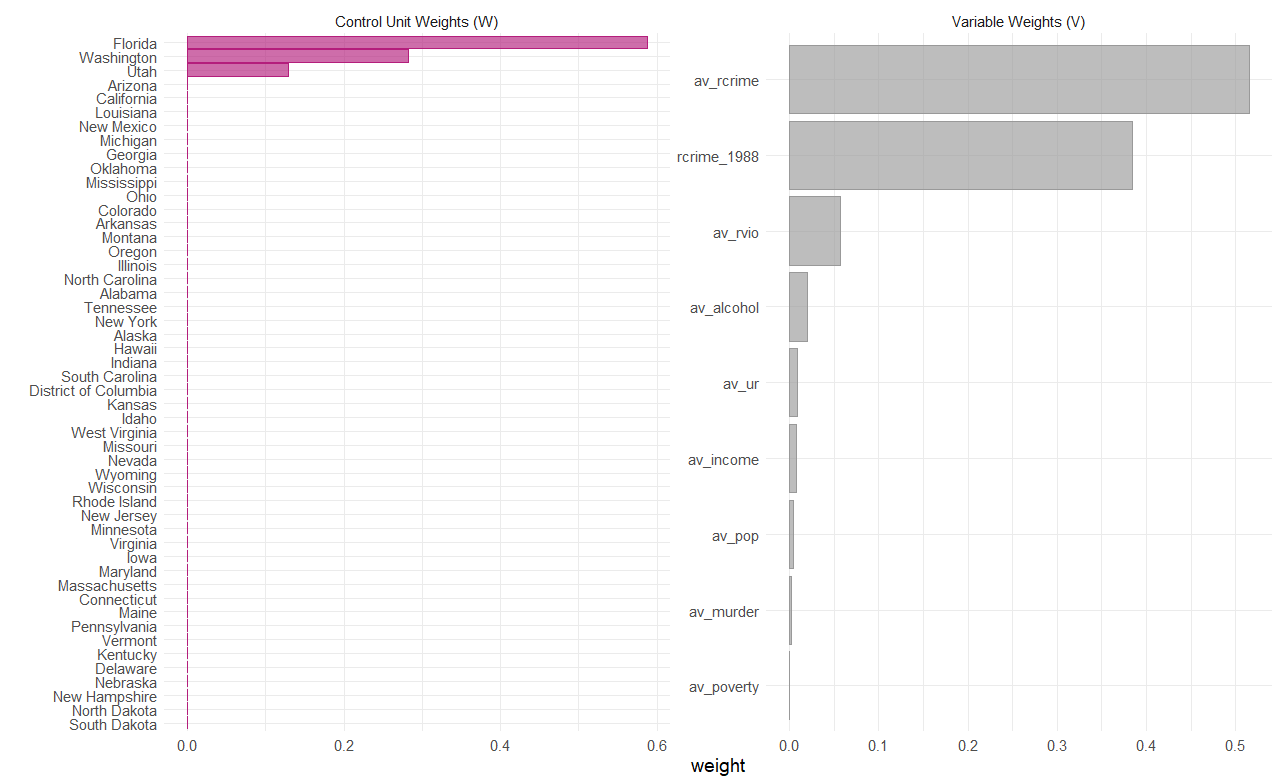
\includegraphics[width=.85\textwidth]{Figures/figure_4.png}
    \end{center}
    \caption{Synthetic Control Weights (after adding variables)}
    \label{fig:graph}
\end{figure}

Personally I don't think Texas is much like Washington State. It's also doubtful that many other states contribute little to the Texas Synthetic trend. The idea is that we should not be overconfident with the estimation of synthetic control.


\begin{figure}[H]
    \begin{center}
        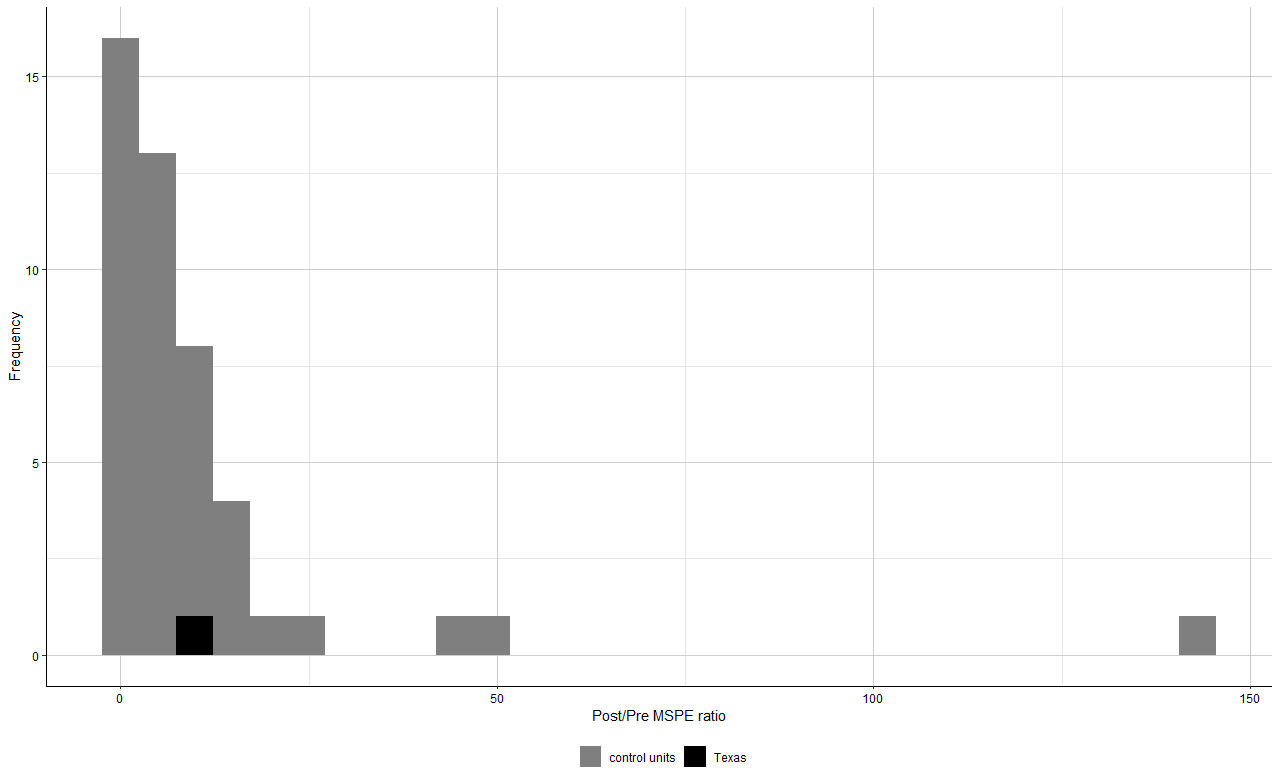
\includegraphics[width=.85\textwidth]{Figures/figure_5.png}
    \end{center}
    \caption{Histogram of the distribution of ratios of post-RMSPE to pre-RMSPE.}
    \label{fig:graph}
\end{figure}


Figure 5 shows the p-value of the estimation. As it shows, the result is insignificant. The placebo distribution in the following figure 6, shows the result similarly. 


\begin{figure}[H]
    \begin{center}
        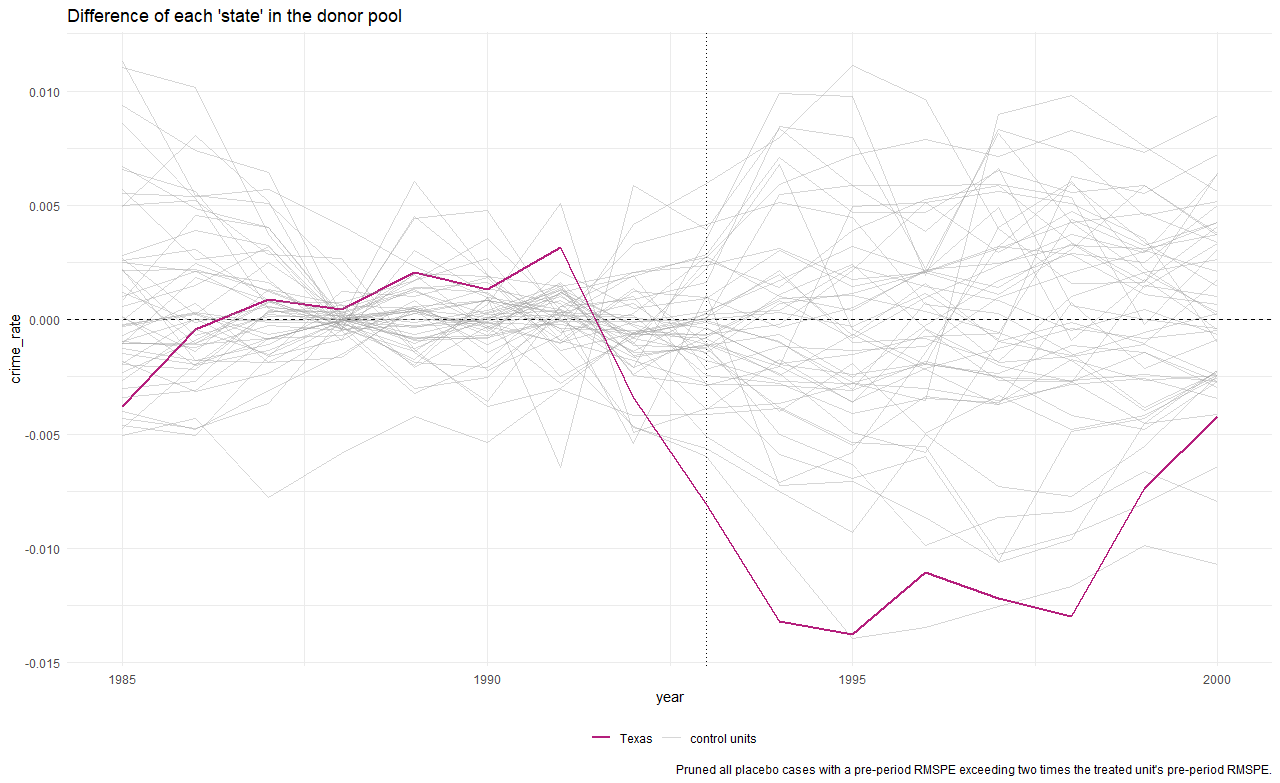
\includegraphics[width=.85\textwidth]{Figures/figure_6.png}
    \end{center}
    \caption{Placebo Distribution}
    \label{fig:graph}
\end{figure}

\section{Conclusion}

The result of synthetic control shows that the treatment effect of building prison is seemingly in short run, and the effect is not significant. From this perspective, constructing prison might not be the best way to deter crime. On the other hand, however, we should not fully trust the synthetic control method, as it remains unknown whether the weights put on different states are appropriate. 

For future work, it would be better to differentiate categories of the crime into different gender, race and age, and check whether the prison construction has more impact on some people. Research of prison construction could also be expanded to the influence of local communities, such as fertility and employment.

\printbibliography[title={References}]


\end{document}